\documentclass{article}
\usepackage{graphicx} % Required for inserting images
\usepackage[margin=1in]{geometry}
\usepackage{amsmath}
\usepackage{amsthm}
\usepackage{amssymb}
\usepackage{amsfonts}
\usepackage{enumitem}
\usepackage{verbatim}
\usepackage{xcolor}
\usepackage{soul}

\title{Homework 6: Report}
\author{Dante Buhl}

\DeclareMathOperator{\cond}{cond}
\DeclareMathOperator{\vecspan}{span}

\begin{document}

\newcommand{\bs}[1]{\boldsymbol{#1}}
\newcommand{\bmp}[1]{\begin{minipage}{#1\textwidth}}
\newcommand{\emp}{\end{minipage}}
\newcommand{\R}{\mathbb{R}}
%\newcommand{\Imag}{\mathbb{I}}
\newcommand{\C}{\mathbb{C}}
\newcommand{\N}{\mathcal{N}}
\newcommand{\I}{\mathrm{I}}
\newcommand{\K}{\bs{\mathrm{K}}}
\newcommand{\m}{\bs{\mu}_*}
\newcommand{\s}{\bs{\Sigma}_*}
\newcommand{\dt}{\Delta t}
\newcommand{\tr}[1]{\text{Tr}(#1)}
\newcommand{\Tr}[1]{\text{Tr}(#1)}

\maketitle

\section*{Question 1: Latency in MPI Communication}

    After modifying the ping pong code from Hw4 and running message size tests
    for double precision real arrays, several plots are produced; one for my personal
    computer, one for hummingbird, and one for lux. The message sizes ranged
    from 1 real to 10000 reals, and each message size was repeated 200 times in
    order to find a significant average for the startup time and the time per
    byte. For each machine used, there is a slightly different plot found,
    however, the general trend is regular. There is some initial slope which is
    fairly linear, for messages below 500-1000 reals (varies for machine), and
    then after that the latency experiences a jump discontinuity or slope
    change and then stays on this slope for the rest of the data sizes with very
    minor deviations. Figures at the end.

    \begin{figure}
        \centering
        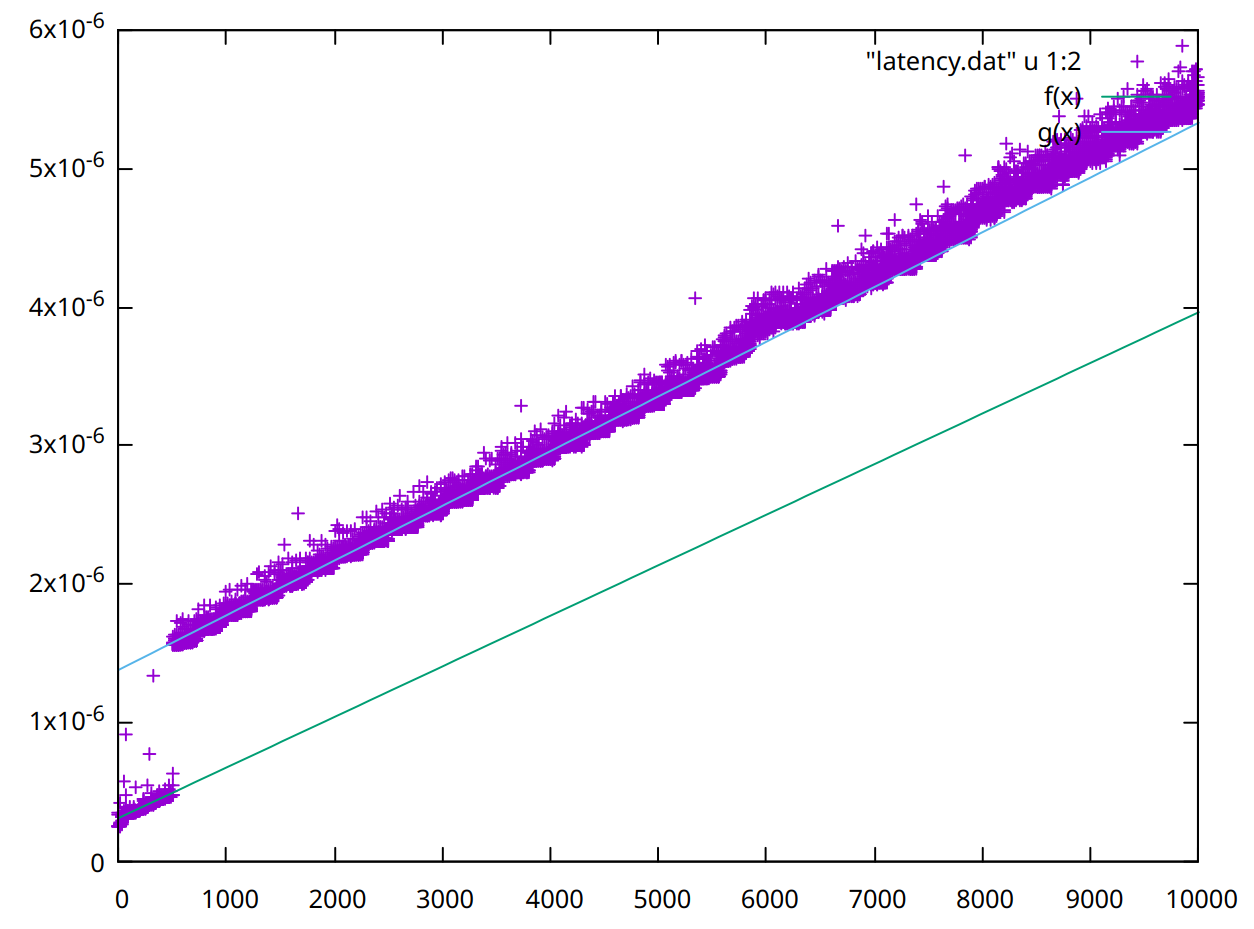
\includegraphics[width=.8\textwidth]{personallatency.png}
        \caption{Latency Plot on my desktop, $t_s = 3.17\cdot10^{-7}$, $t_w =
        3.64\cdot10^{-10}$}
    \end{figure}

    \begin{figure}
        \centering
        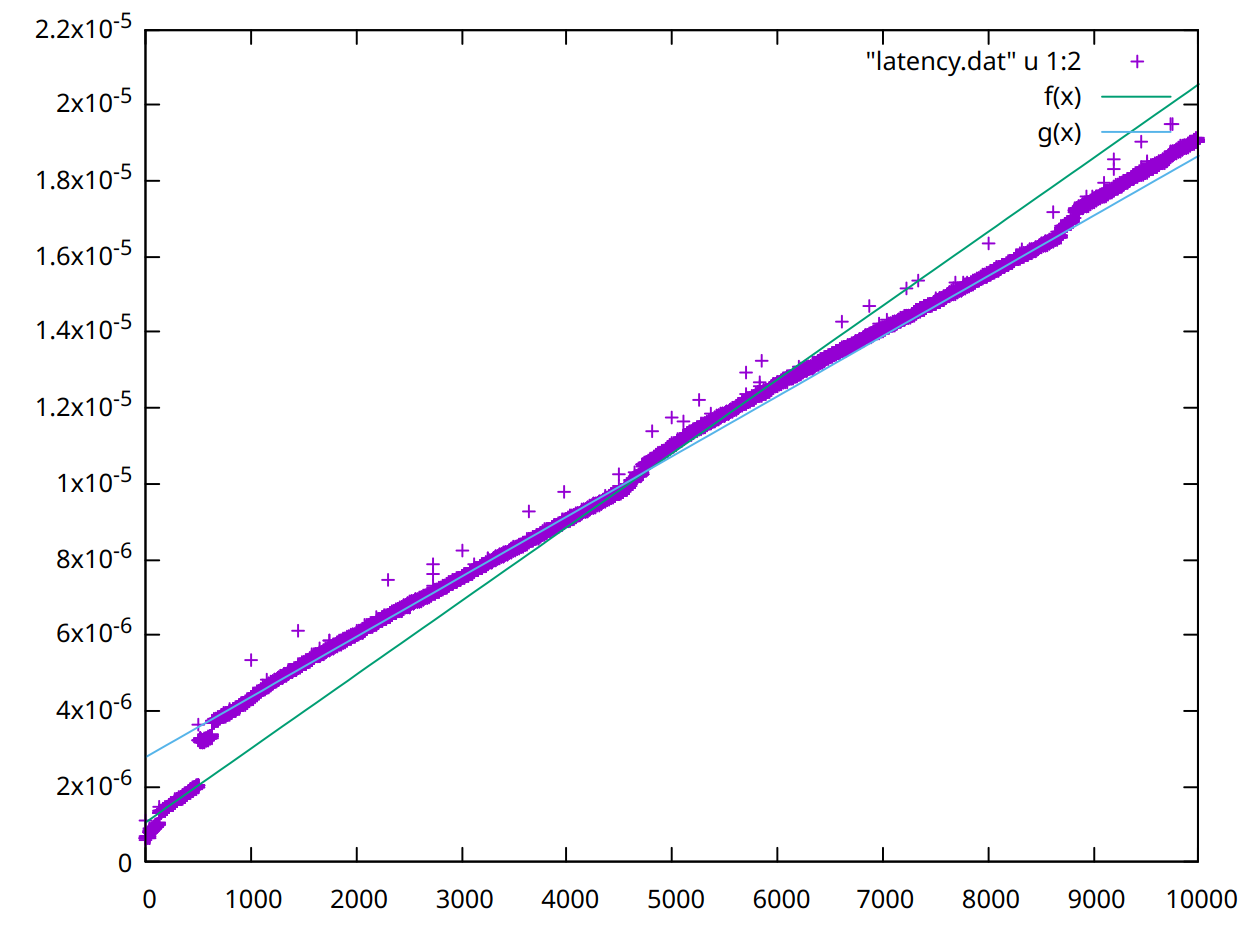
\includegraphics[width=.8\textwidth]{hblatency.png}
        \caption{Latency Plot on Hummingbird, $t_s = 1.05\cdot10^{-6}$, $t_w =
        1.58826\cdot10^{-9}$}
    \end{figure}

    \begin{figure}
        \centering
        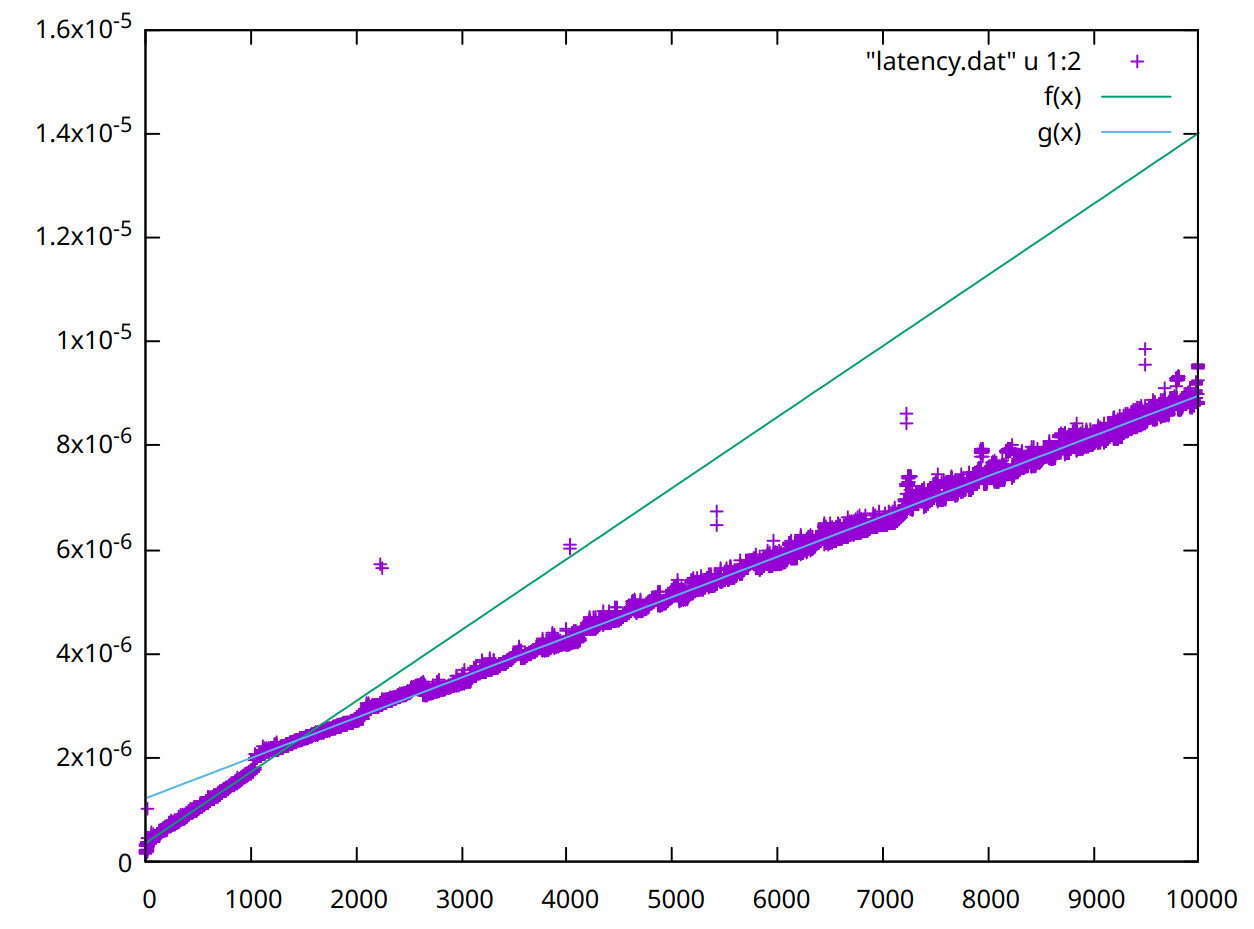
\includegraphics[width=.8\textwidth]{luxlatency.png}
        \caption{Latency Plot on Lux, $t_s = 3.70\cdot10^{-7}$, $t_w =
        7.73\cdot10^{-10}$}
    \end{figure}

              
               
\section*{Question 2: Finite Difference Stencil}
    For this problem, the only part that changes is that we decompose the
    domain in to pencils instead of planes. This changes the communication
    structure but doesn't force us to change the computation time. 
    We see that instead of communicating  $NN_z$ cells in 2 directions we communicate
    $N_z$ cells in 4 directions. This means that the communication startup will impact the
    execution time more than before, but it also allows the isoefficiency to be
    $O(P)$. 
    \setcounter{section}{2}
    \subsection{\textbf{Execution Time}}
    \[
        T_{2D\_FD} = \frac{T_{comm} + T_{comp}}{P}
    \]
    \[
        T_{comp} = t_c N^2N_z, \quad T_{comm} = 4P(t_s + 2t_wN_z)
    \]
    \[
        T_{2D\_FD} = \frac{t_cN^2N_z}{P} + 4t_s + 8t_wN_z
    \]
    \subsection{\textbf{Efficiency}}
    \[
        E = \frac{T_1}{PT_{2D\_FD}} = \frac{t_cN^2N_z}{t_cN^2N_z + 4Pt_s + 8t_wN_zP}
    \]

    \subsection{\textbf{Isoefficiency}}
    \[
        E = C \implies t_cN^2N_z = E(t_cN^2N_z + 4Pt_s + 8t_wN_zP)
    \]
    \[
        N^2 \sim P \implies t_cN_z = E(t_cN_z + 4t_s + 8t_wN_z)
    \]
    \[
        \text{Isoefficiency} \sim O(P)
    \]
    Obviously this isoefficiency is better than the one presented in the lecture
    note. We see that though we my communicate more, we see that we only have to
    scale the domain by the square root of the number of processors implying
    better isoefficiency. 


\end{document}


